\chapter{\des}
  \section{Beskrivelse/teori}
    \fxnote[inline]{Beskrivelse af tidsmodellen, teorien omkring den og 
    hvor/hvad den benyttes til. Teori: henvisning til litteratur, bl.a.  
    matematik/beviser for modellen}
    
\subsection*{Barrierer}\label{barrier}
For at modellere tid i PyCSP, skal der foretages en 
række valg. I \des findes der i modsætningen til 
Parallel \des \fixme{referencer} en global tid og alle processerne skal derfor have  en 
fælles tid der tæller op samtidigt. Den mest brugte metode i CSP sammenhæng er 
at implementere en barrier som en selvstændig process. Eksempelvis kan den implementers som i \autoref{barrier-imp}.
%\begin{minipage}[b]{1\linewidth}

\begin{lstlisting}[float, label=barrier-imp,caption=En barrier i PyCSP]
@process
def Barrier(nprocesses, signalIN, signalOUT):
	while True:
		for i in range (nprocesses):
			signalIN()
		for i in range (nprocesses):
			signalOUT(0)
\end{lstlisting}
%\end{minipage}

Barrier blev introduceret i MPI, og sikrer at alle tråde har nået dette punkt 
før de må fortsætte. I PyCSP er det trivielt at have  denne egenskab, da 
processer til begge kanalender er klar, og med to kanaler kan man sikre at 
ingen proces modtager et signal før alle processer har sendt et signal til 
barrieren.
\fxnote[inline]{fortsættes med ulemper med barriere og generelt hvorfor vi 
skal holdes os fra det. noget med at man skal kalde barrieren to  gange}

\section{Eksempel}
\fxnote[inline]{Beskrivelse af eksemplet og hvordan det er relateret til problemet/modellen. Beskrivelse af løsning uden vores tid}


\subsection{Hajer og fisk på Wator} Som eksempel på en \des har vi valgt at tage 
udgangspunkt i det scenarie som A. K. Dewdney
beskrev i artiklen \cite{wator}. Artiklen beskriver den
fiktive planet Wator, der har form som en torus og er fuldstændig
dækket af vand. Verdenen er inddelt i felter \cite[s. 20]{wator}, og disse felter kan være tomme, indeholde en
fisk eller en haj. Følgende karakteristika beskriver fisk og hajers
opførsel.

\begin{itemize}
\item[Fisk]
Lever af plankton, en ressource som er uendelig. Hvis der er en ledigt 
tilstødende felt, bevæger en fisk sig til dette felt. Hvis der er flere ledige 
felter vælges et tilfældigt. Såfremt en fisk overlever 3 tidsskridt forplanter 
den sig.
\item[Hajer]
Såfremt der er fisk i et eller flere tilstødende felter, vil hajen bevæge sig 
til et af disse felter og spise fisken. Hvis der er ikke er nogen fisk i et af 
disse felter flytter hajen sig til et tilfældigt valgt ledigt felt. Hvis en haj 
ikke spiser i 3 tidsskridt dør den. Overlever den i 10 tidsskridt forplanter 
den sig.
\end{itemize}

For hvert tidsskridt vil alle fisk og hajer udføre en handling ud fra
ovenstående opførsel.
Til at initiere systemet skal der defineres en størrelse af verdenen,
samt hvor mange fisk og hajer der er til stede fra start. Disse fisk og
hajer placeres tilfældigt i verdenen.
Såfremt de initielle parametre for antal fisk og hajer understøtter en 
bæredygtig bestand forventer vi at se bestanden af henholdsvis fisk og hajer 
oscillerer afhængigt af hinanden.

\fxnote[inline]{Hvorfor har vi valgt dette eksempel. Hvorfor er dette eksempel 
relevant til brug i parallel computing. Hvorfor forventer vi at det kan gøres 
smartere med introdsuktionen af tid.}

Vi har valgt dette eksempel, da det er enkelt og let forståeligt, men samtidig 
introducerer problemstilinger omkring synkronisering når det paralleliseres.  
Disse problemstillinger optræder fordi en opdatering af hvert felt er afhængigt 
af de omkringliggende felter, og vil derfor være afhængig af felter fra andre 
processer i grænsetilfælde. Ud over at være afhængig af information fra andre 
processer, kan en opdatering også påvirke data hos andre processer. Dette er 
tilfældet hvis en fisk eller haj skal bevæge sig fra et område styret af èn 
proces til et område styret af en anden proces.  \fxnote[inline]{Noget om real 
world applikation?}

\subsubsection*{Før introduktion af et tidsbegreb i CSP} 
For at simulere Wator verdenen i et CSP-system hvori tidsbegrebet ikke er 
introduceret, er vi nødt til at udføre en synkronisering af de enkelte 
processers arbejde. Denne synkronisering kan ske ved brug af barrierer, hvor 
alle processer udfører en handling og mødes i barrieren før de fortsætter.

\fxnote[inline]{MAV af model, hvorfor ikke en bedre csp approch med forsendelse 
af shadowrows og totalt seperapelt data}
Vi har valgt at basere vores model på \cite{crew}, hvor verdenen repræsenteres 
som en delt datastruktur og adgangen til denne styres med barrierer. I vores 
model er hver proces derved ansvarlig for en del af verdenen og tilgangen til 
den delte datastruktur sker ud fra CREW-princippet (Concurrent Read, Exclusive 
Write) som angivet i artiklen, og styres vha. af barrierer. 

Vi deler verdenen lodret, hvor hver proces styrer en verdensdel. Hver proces 
gennemgår sin verdensdel og udfører en mulig handling for hver fisk og haj, dog 
vil fisk og hajer i de sidste to kolonner i hver verdensdel ikke bliver 
opdateret på nuværende tidspunkt. Dette skyldes at henholdsvis processen selv 
og den umiddelbar til højre for den, har skriverettigheder til disse to 
kolonner.
Når denne opdatering er fuldført mødes processerne i en barriere, hvorefter 
hver proces opdaterer de to sidste kolonner. Herefter mødes processerne igen i 
barrieren, og når alle kolonner er opdateret, kan der foretages en 
visualisering af de udførte opdateringer. Til slut mødes alle i en barrierer igen før processerne kan begynde en ny iteration \fxnote[inline]{pseudo kode eksempel?}

En representation af opdelingen ses på \autoref{fig:wator}. Her er verdenen 
opdelt mellem to processer, og de to kolonner mellem hver del opdateres i et 
seperat tidsskridt. Når disse to tidsskridt er udført kan der foretages en 
visualisering, hovrefter næste iteration af opdateringer kan begyndes.  

Vi har valgt denne model frem for en mere ren CSP model, da denne model 
klarlægger brugen af barrierer bedre. I en mere ren CSP-model ville man 
foretage en direkte udveksling af data mellem 
processerne,\fxnote[inline]{mere\ldots} 

\fxnote{konklusion hvordan var det at implementerer og hvor stor parallelitet kan man opnå. }

\begin{figure}[hbtp]
  \begin{center}
  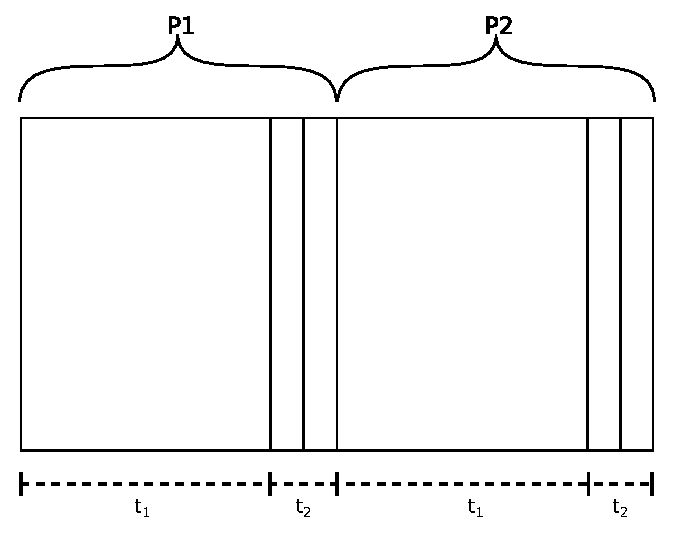
\includegraphics[scale=0.75]{images/wator}
  \caption{Opdeling af verdenen mellem to processer. Der er for hver verdensdel 
  to kolonner som opdateres i et seperat tidsskridt.}
  \label{fig:wator}
  \end{center}
\end{figure}

\subsection{Kunder i en bank} Et klassisk eksempel inden for \des er at simulere  
en række kunder der alle ankommer til en butik, hvor de skal serviceres. Dette 
simple problem kan bruges til at modellere mange forskellige 
problemstillinger, som hvordan flowet ændrer sig hvis man varier en parameter 
i systemet. Programmeringssproget SimPy\fxnote{ref} har som et af deres eksempel, en 
simulering af kunder i en bank. SimPy bruger dette som en gennemgående 
eksempler hvor de løbende udvider deres model for at vise forskellige 
egenskaber ved deres model. For senere at kunne sammenligne SimPy  med vores 
implementation af logisk tid vil vi implementere to af SimPYs eksempler i PyCSP.

I det simple tilfælde af eksemplet ankommer der en kunde til banken på på et 
tilfældigt tidspunkt. Hun opholder sig i banken i et tidsrum, hvorefter hun 
igen forlader banken.

I det simple eksempel kan der ikke uddrages meget information, men det viser hvordan en simpel model er opbygget for at håndtere tid.
I det andet eksempel er modellen 
udvidet med en service disk. Her skal alle kunderne betjenes af en 
servicemedarbejder, som kun kan ekspedere en kunde af gangen. Alle kunder ankommer til banken i tilfældig orden og 
stiller sig i kø til at blive serviceret. Dette  svare til en M/M/1\fixme{hvad  
er en m/m/1 kø} kø. Dette er stadigt en meget simpel model, men ud fra køen kan der måles hvor lang tid det tager i gennemsnit for kunderne at blive betjent af servicemedarbejdere, samt hvor lang køen er over tid. 

\subsubsection{Før introduktion af et tidsbegreb i PyCSP}
I SimPy er kunderne en proces og det vil derfor være nærliggende ligeledes at 
modellere eksemplet i PyCSP med kunder som en proces. i SimPy kalder 
generatorfunktionen kunderne og kan kører den parallelt med sig selv. 
I PyCSP\fxnote{hvorfor?- kan man lave child processes der køre i samme 
parallel kald som dets parent?}, er standard metoden\fxnote{set fra 
kodeeksempler} at modellere mere statiske objekter, med en source og sink 
process og lade arbejdet flyttes mellem processerne. Derfor er modellen ændret 
så  generatorprocesen stadigt fungere som en source, men vi introducerer en 
bankproces som sink, og lader kunderne være arbejdet der flyttes mellem dem. 

Mens SimPy  kalder kundeprocessen og lader denne stå for håndteringen af 
kunden og tiden hun befinder sig i banken, har bankprocessen i PyCSP ikke 
mulighed for at kende tid og skal derfor selv holde en liste med kunderne 
i banken og  til hver tidskridt vide hvilke af kunderne der skal forlade 
banken. 

Tiden er igen modelleret ved brug af barrier se afsnit \vref{barrier}, men 
i stedet for  at kalde barrierens to krævede kald, lige efter hinanden, som 
normalt, for at være sikker på vi er i samme tidsskridt lader vi bank
processen gå ind i barrieren i starten af tidsskridtet, og så modtage kunder, 
indtil banken modtager et kald om at forsætte til næste tidsskridt af 
barrieren (se \autoref{bank-alternation-imp}). Dette er smart, og nødvendigt for at lade banken have mulighed for at modtage 
et vilkårligt antal kunder i samme tidsskridt, samt vide hvornår der ikke vil  
komme flere kunder. Vi kan ressonere os til at barrieren stadigt virker efter 
hensigten ved at indse at for at generatoren kan komme foran med et tidsskridt og sende en 
kunde i et forkert tidsskridt skal den have fuldført begge begge kald til barrieren, men 
barrieren vil ikke modtage et kald fra nogle før det har kaldt bankprocessen, 
og derfor må generatoren vente i sit første kald til barrieren indtil banken har 
modtaget sit kald fra barrieren. 

\begin{lstlisting}[float=hbtp,label=bank-alternation-imp,caption=Modtage en kunde eller 
	barrier i Bankprocessen]
while True:
		(g,msg) = Alternation([{
		barrierREADER:None,
    customerREADER:None
    }]).select()
		if g == barrierREADER:
			break
    elif g == customerREADER:
			heappush(customers,(time+msg.waittime,msg))
\end{lstlisting}


Da dette eksempel er taget fra SimPy, for at vise fordelene ved simulering, egner det sig selvfølgelig godt til simulering, og fra eksemplet kan man også se at der findes meget kode til bookkeping, som eksmplerne i SimPY ikke har. Det drejer sig om kode der sørge for at hver proces kender tiden, samt at den er synkroniseret på tværs af processerne. Vi forventer derfor at koden skal kunne simplificeres i PyCSP med tid, så det bliver lige så simpelt som i SimPY.

I det mere avancerede eksempel hvor kunderne skal tilgå den samme begrænsede ressource dannes en kø. Denne kan i PyCSP modeleres på flere måder, afhængigt at hvilken proces der skal have ansvaret for at vedligeholde køen. En metode er internt i en proces at have en liste, og lade det være processens ansvar at håndtere køen. Processen med ansvaret kan så enten være den begrænsede ressource, eller en separat proces hvis eneste formål er at vedligeholde køen. For nyligt er der i PyCSP blevet introduceret ''buffered channels'', og disse kan også bruges som en kø. Dermed kan man modellere sin ressource og lade den læse fra kanalen når den er klar uden at skulle beskæftige sig med køen, og uden at skulle implementerer en hjælper proces til håndtering af køen. Vi har i dette eksempel valgt at lade køen være repræsenteret ved en ''buffered channel'', men den kunne lige så godt være repræsenteret som en liste i servicedisk processen.

I SimPy findes begrebet ressource direkte i sproget som en type og servicedisken er blot en instans af denne type, og ressourcen står selv for at håndterer køen. I PyCSP modelleres servicedisken som en separat proces, og bankprocessen er reduceret til blot at sende kunden videre til servicedisken og lade kanalen håndtere køen. En ulempe ved denne implementation er dog at kanalen har en fast størrelse på sin buffer, og dermed riskere man ved brug af buffers og barrierer en deadlock hvis ikke processen i samme tidsskridt kan foretage transmissionen og kalde barrieren. det kan du løses med en alternation og skip guard, men så skal banken håndtere fejlede forsendelser og må introducere en sekundær kø hvilket gør at introduktionen af en ''buffered channel'' er irrelevant. Vi har valgt blot at angive en maksimal størrelse på bufferen som er større end det totale antal kunder banken modtager.

ULEMPER MED BARRIER:
En stor ulempe ved den simple form for barrierer er at antallet af processer skal være konstant gennem hele kørslen.

Dette er f.eks. et problem i bank eksmplet hvor generatorfunktionen kan slutte lige efter at have genereret den sidste kunde, og før denne er færdig processeret af servicedisken. Her må den nødvændigvis fortsætte indtil alle processer kan slutte. Alternativt må barrierprocessen ændres så den dynamisk kan ændre på hvor mange processer der skal synkroniseres.


  \section{Design og implementation}
    \fxnote[inline]{Beskrivelse af design med udgangspunkt i eksemplet}
    \section{Repræcentation af tid}

I PyCSP foregår kommunikation kun når begge kanalender er klar dvs.
når der findes både en kanalende der vil skrive og en kanalende der vil læse. 
Hvis kun en af kanalenderne er klar, vil den vente indtil
der findes minumum en kanalende af hver type, der er klar. I alternation 
findes muligheden for at tilknytte en timeout til en guard. Dette
giver muligheden for at en process, kun er villig til at vente på at kanalen 
bliver klar inden for en given tidsperiode. 
\begin{lstlisting}[label=Timeout,
  caption=Timeout i Alternation (fra dokumentationen til PyCSP)]
  Alternation([{Timeout(seconds=0.5):None},
               {Cin:None}]).select()
\end{lstlisting} 

I denne alternation er processen villig til at læse fra Cin i 0.5 sekunder. 
Ellers accepteres timeoutguarden og processen er ikke længere villig til at 
læse fra Cin.

Med et simuleringsmiljø er det ikke nok udelukkende kan kunne specifiere en 
timeout på kanalen, det er også nødvændigt at man kan specificere at en proces 
er villig til at kommunikere fra et tidspunkt, samt at den kanalen kun er 
villig til at kommunikere på nuværende tidpunkt, men ikke ud i fremtiden. 

At ville kommunikere fra et given tidspunkt i fremtiden,  svare til at vente 
uden at lave noget indtil det givne tidspunkt for så at forsøge at kommunikere 
fra tidpunktet indtil det kommunktationen lykedes. Dette kan dermed laves helt 
uden en alternation, men ved blot med de to funktioner Wait(time), Cin(). 

At ville være villig til at kommuikere til et given tidspunkt, medfører en ny 
problemstilling, da det introducere muligheden for deadlocks og 
nondeterminisme\fxnote{Er det korrekt?}, for det er ikke defineret hvad tiden 
er hvis det ikke lykkedes at kommunikere i det givne tidsskridt. Der findes to 
muligheder, enten skal scheduleren signalere at der ikke findes mere arbejde 
til dette tidsskridt, og lade processerne fortsætte i samme tidsskridt. 
Alternativt skal tiden tælles op til næste event, hvorefter processerne 
signaleres med at kommunkationen ikke lykkedes. Hvis processerne signalleres 
i samme tidsskridt kan man vælge enten at signallere hver proces en af gangen 
eller samtidigt at signallerer alle processerne. ingen af mulig

processen fortsætte  tildet under antagelsen af problemer.




når tiden er  tidspunkt
til for et findes der allerede \fxnote[inline]{vi skal kunne angive
at vi ønsker at kommunikere men KUN i det tidsskridt vi er i, og at
hvis dette ikke kan lade sig gøre skal vi breake noget alla at have en
timeout på 0} 

  \section{Evaluering}
    \fxnote[inline]{Evaluering af hvordan eksemplet løses efter den valgte 
    implementation benyttes. Inkluderer test+performance}
  \section{Fremtidigt arbejde}
  \section{Opsummering}
